\documentclass[11pt,a4paper]{article}

% --- Core Packages ---
\usepackage[utf8]{inputenc}
\usepackage[T1]{fontenc}
\usepackage[english]{babel}
\usepackage{geometry}
\usepackage{xcolor}
\usepackage{amsmath,amssymb,amsfonts,mathtools}
\usepackage{booktabs,tabularx,array,multirow}
\usepackage{listings}
\usepackage{tikz}
\usetikzlibrary{arrows.meta,positioning,shapes.geometric,calc,decorations.pathreplacing,trees,backgrounds}
\usepackage{tcolorbox}
\tcbuselibrary{skins,theorems}
\usepackage{fancyhdr}
\usepackage{titlesec}
\usepackage{enumitem}
\usepackage{parskip}
\usepackage{lastpage}
\usepackage{hyperref}

% --- Page Geometry ---
\geometry{
    top=2.2cm,
    bottom=2.2cm,
    left=2.2cm,
    right=2.2cm,
    headheight=22pt
}

% --- Color Palette (Matching Course Theme) ---
\definecolor{ForestGreen}{RGB}{22,100,70}
\definecolor{DeepGreen}{RGB}{14,70,48}
\definecolor{SoftGreen}{RGB}{238,247,242}
\definecolor{DarkBlue}{RGB}{20,50,110}
\definecolor{SoftBlue}{RGB}{236,243,253}
\definecolor{DarkOrange}{RGB}{180,85,15}
\definecolor{SoftOrange}{RGB}{254,246,236}
\definecolor{SoftPurple}{RGB}{245,240,254}
\definecolor{DarkPurple}{RGB}{90,40,140}
\definecolor{CodeBg}{RGB}{248,250,249}
\definecolor{BorderGray}{RGB}{210,218,214}
\definecolor{DarkGray}{RGB}{50,50,50}

% --- Hyperref Setup ---
\hypersetup{
    colorlinks=true,
    linkcolor=DeepGreen,
    citecolor=DarkBlue,
    urlcolor=ForestGreen,
    pdftitle={DSAI1002 Lecture Notes - Part 04: Sorting, Selection, and Searching Algorithms},
    pdfauthor={Dr. Minh D. Vu - NEU}
}

% --- Fancyhdr Header/Footer ---
\pagestyle{fancy}
\fancyhf{}
\fancyhead[L]{\small\textbf{\color{ForestGreen}DSAI1002 -- Data Structures and Algorithms with Python}}
\fancyhead[R]{\small\color{DarkGray}Lecture Notes -- Part 04}
\fancyfoot[L]{\small\color{DarkGray}Instructor: Dr. Minh D. Vu}
\fancyfoot[R]{\small\color{DarkGray}Page \thepage\ of \pageref{LastPage}}
\renewcommand{\headrulewidth}{0.5pt}
\renewcommand{\headrule}{\hbox to\headwidth{\color{ForestGreen}\leaders\hrule height \headrulewidth\hfill}}
\renewcommand{\footrulewidth}{0.3pt}
\renewcommand{\footrule}{\hbox to\headwidth{\color{BorderGray}\leaders\hrule height \footrulewidth\hfill}}

% --- Section Styling ---
\titleformat{\section}
  {\Large\bfseries\color{DeepGreen}}
  {\thesection.}{0.6em}{}
  [{\color{ForestGreen}\titlerule[1pt]}]

\titleformat{\subsection}
  {\large\bfseries\color{ForestGreen}}
  {\thesubsection}{0.5em}{}

\titleformat{\subsubsection}
  {\normalsize\bfseries\color{DarkBlue}}
  {\thesubsubsection}{0.4em}{}

% --- Custom Tcolorboxes ---
\newtcolorbox{definitionbox}[1][]{
    enhanced,
    colback=SoftBlue,
    colframe=DarkBlue,
    boxrule=0.8pt,
    arc=2mm,
    left=3mm, right=3mm, top=2.5mm, bottom=2.5mm,
    title=\textbf{\color{DarkBlue}#1},
    coltitle=DarkBlue,
    attach boxed title to top left={yshift=-2mm, xshift=3mm},
    boxed title style={colback=white, boxrule=0.6pt, colframe=DarkBlue, arc=1mm}
}

\newtcolorbox{theorembox}[1][]{
    enhanced,
    colback=SoftGreen,
    colframe=ForestGreen,
    boxrule=0.8pt,
    arc=2mm,
    left=3mm, right=3mm, top=2.5mm, bottom=2.5mm,
    title=\textbf{\color{ForestGreen}#1},
    coltitle=ForestGreen,
    attach boxed title to top left={yshift=-2mm, xshift=3mm},
    boxed title style={colback=white, boxrule=0.6pt, colframe=ForestGreen, arc=1mm}
}

\newtcolorbox{examplebox}[1][]{
    enhanced,
    colback=SoftOrange,
    colframe=DarkOrange,
    boxrule=0.8pt,
    arc=2mm,
    left=3mm, right=3mm, top=2.5mm, bottom=2.5mm,
    title=\textbf{\color{DarkOrange}#1},
    coltitle=DarkOrange,
    attach boxed title to top left={yshift=-2mm, xshift=3mm},
    boxed title style={colback=white, boxrule=0.6pt, colframe=DarkOrange, arc=1mm}
}

\newtcolorbox{notebox}[1][]{
    enhanced,
    colback=SoftPurple,
    colframe=DarkPurple,
    boxrule=0.8pt,
    arc=2mm,
    left=3mm, right=3mm, top=2.5mm, bottom=2.5mm,
    title=\textbf{\color{DarkPurple}#1},
    coltitle=DarkPurple,
    attach boxed title to top left={yshift=-2mm, xshift=3mm},
    boxed title style={colback=white, boxrule=0.6pt, colframe=DarkPurple, arc=1mm}
}

% --- Code Listings Setup ---
\lstdefinestyle{pythonstyle}{
    language=Python,
    basicstyle=\ttfamily\footnotesize,
    keywordstyle=\color{DarkBlue}\bfseries,
    stringstyle=\color{red!70!black},
    commentstyle=\color{ForestGreen}\itshape,
    numberstyle=\tiny\color{gray},
    numbers=left,
    numbersep=7pt,
    frame=single,
    rulecolor=\color{BorderGray},
    backgroundcolor=\color{CodeBg},
    breaklines=true,
    breakatwhitespace=true,
    tabsize=4,
    showstringspaces=false,
    columns=fullflexible,
    keepspaces=true,
    xleftmargin=1.5em,
    aboveskip=0.6em,
    belowskip=0.6em
}

\lstdefinestyle{pseudostyle}{
    language={},
    basicstyle=\ttfamily\footnotesize,
    keywordstyle=\color{DarkBlue}\bfseries,
    morekeywords={ALGORITHM,FUNCTION,INPUT,OUTPUT,IF,THEN,ELSE,ELSEIF,RETURN,FOR,TO,DOWNTO,DO,WHILE,REPEAT,UNTIL,TRUE,FALSE,AND,OR,NOT,SWAP,LENGTH,APPEND,DIV,MOD,CREATE,NONE},
    numberstyle=\tiny\color{gray},
    numbers=left,
    numbersep=7pt,
    frame=single,
    rulecolor=\color{ForestGreen!40},
    backgroundcolor=\color{CodeBg},
    breaklines=true,
    tabsize=4,
    showstringspaces=false,
    columns=fullflexible,
    keepspaces=true,
    xleftmargin=1.5em,
    aboveskip=0.6em,
    belowskip=0.6em
}

\lstset{style=pythonstyle}

% --- Custom TikZ Styles for Array Trace ---
\tikzset{
  cell/.style={draw=ForestGreen,fill=SoftGreen,thick,minimum width=0.82cm,minimum height=0.72cm,align=center},
  active/.style={draw=DarkOrange,fill=SoftOrange,very thick,minimum width=0.82cm,minimum height=0.72cm,align=center},
  pivot/.style={draw=DarkPurple,fill=SoftPurple,very thick,minimum width=0.82cm,minimum height=0.72cm,align=center},
  cellgray/.style={draw=gray,fill=black!5,thick,minimum width=0.82cm,minimum height=0.72cm,align=center}
}

% =========================================================================
% DOCUMENT BEGINS
% =========================================================================
\begin{document}

% --- TITLE BANNER ---
\begin{tcolorbox}[
    enhanced,
    colback=SoftGreen,
    colframe=ForestGreen,
    boxrule=1.5pt,
    arc=3mm,
    left=5mm, right=5mm, top=6mm, bottom=6mm
]
\begin{center}
    {\Large\scshape National Economics University -- Faculty of Data Science and AI}\\[0.3em]
    {\large\textbf{\color{DarkBlue}DSAI1002: Data Structures and Algorithms with Python}}\\[0.8em]
    {\Huge\bfseries\color{ForestGreen} LECTURE NOTES: PART 04}\\[0.4em]
    {\LARGE\bfseries\color{DarkGray} Sorting, Selection, and Searching Algorithms}\\[0.8em]
    \rule{0.7\textwidth}{0.8pt}\\[0.6em]
    {\normalsize\textbf{Author / Instructor:} Dr. Minh D. Vu \quad$|$\quad \textbf{Term:} Fall 2026}\\[0.2em]
    {\small\textit{Comprehensive Academic Monograph on Sorting Models, Comparison vs. Non-Comparison Algorithms, Order Statistics, Binary/Ternary Searching, and Practical Python Integration}}
\end{center}
\end{tcolorbox}

\vspace{0.5em}

% --- EXECUTIVE SUMMARY ---
\begin{notebox}[Executive Roadmap of Part 04]
This monograph synthesizes the theoretical concepts, formal algorithms, step-by-step traces, and complexity analyses presented across \textbf{Lecture 4}:
\begin{enumerate}[itemsep=1pt,topsep=2pt]
    \item \textbf{Foundations of Sorting:} Motivation, mathematical specification, core taxonomy (stability, in-place, adaptiveness, online vs. offline, comparison vs. integer-key).
    \item \textbf{Elementary Comparison Sorts:} Insertion Sort (card-hand model, loop invariant, $\Theta(n)$ best case, $\Theta(n^2)$ worst case) and Bubble Sort (adjacent swaps, early termination flag, $\Theta(n^2)$ worst case).
    \item \textbf{Divide-and-Conquer Sorting:} Merge Sort (two-way merge buffer, $\Theta(n \log n)$ guaranteed, stability, $O(n)$ extra space) and Quick Sort (Lomuto partition, pivot selection strategies, worst-case avoidance, expected $O(n \log n)$ in-place).
    \item \textbf{Non-Comparison Linear Sorts:} The $\Omega(n \log n)$ decision tree lower bound, Counting Sort ($\Theta(n+k)$ stable index mapping), and Radix Sort (multi-pass LSD stable digit distribution, $\Theta(d(n+b))$).
    \item \textbf{Python Sorting Ecosystem:} Timsort mechanics, `sorted()` vs. `list.sort()`, multi-key ranking, lambda keys, and common sorting bugs.
    \item \textbf{The Selection Problem:} Order statistics, extreme values, Quickselect (expected $\Theta(n)$ average rank retrieval), the Median of Medians algorithm (deterministic $O(n)$ worst case), and Top-$k$ strategies.
    \item \textbf{Searching Algorithms \& Optimization:} Linear search, Binary Search (invariants, overflow avoidance, first/last occurrence variants, `bisect`), Ternary Search on unimodal functions and discrete arrays, and data structure selection tradeoffs.
\end{enumerate}
\end{notebox}

\tableofcontents
\newpage

% =========================================================================
\section{The Sorting Problem and Core Algorithmic Properties}
% =========================================================================

\subsection{Why Study Sorting Algorithms?}
In computational systems, raw data rarely arrives in an organized manner. Sorting rearranges items into a predictable sequence. While sorting is rarely an end in itself, it functions as a critical foundational utility:
\begin{itemize}[itemsep=2pt]
    \item \textbf{Search Acceleration:} In an unsorted array of size $n$, finding an item requires linear search ($O(n)$). Once sorted, searching requires only $O(\log n)$ via binary search (reducing 1,000,000 checks to just 20 comparisons).
    \item \textbf{Duplicate Detection:} In unsorted data, detecting duplicates takes $O(n^2)$ naive checks or extra hash tables. In sorted data, identical elements are contiguous and can be found in a single $O(n)$ pass.
    \item \textbf{Database and Index Operations:} Relational joins (Merge Join), grouping, and range queries rely fundamentally on sorted inputs.
    \item \textbf{Ubiquitous Applications:} E-commerce product listings (by price or rating), financial transactions (chronological audit trails), student GPA rankings, and airline flight departures.
\end{itemize}

\begin{center}
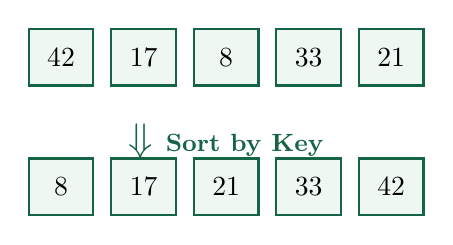
\begin{tikzpicture}[node distance=0.2cm]
\node[cell] (a1) {42};
\node[cell,right=of a1] (a2) {17};
\node[cell,right=of a2] (a3) {8};
\node[cell,right=of a3] (a4) {33};
\node[cell,right=of a4] (a5) {21};

\node[below=0.35cm of a3,font=\Large,ForestGreen] (arr) {$\Downarrow$ \small\textbf{Sort by Key}};

\node[cell,below=0.9cm of a1] (b1) {8};
\node[cell,right=of b1] (b2) {17};
\node[cell,right=of b2] (b3) {21};
\node[cell,right=of b3] (b4) {33};
\node[cell,right=of b4] (b5) {42};
\end{tikzpicture}
\end{center}

\subsection{Formal Mathematical Problem Specification}

\begin{definitionbox}[Definition 1.1 (The Sorting Problem)]
Given an input sequence of $n$ records $A = \langle a_0, a_1, \dots, a_{n-1} \rangle$ and a key extraction function $k: A \to \mathcal{K}$ associated with a total ordering relation $\le$ on $\mathcal{K}$, compute a permutation $A' = \langle a'_0, a'_1, \dots, a'_{n-1} \rangle$ of $A$ such that:
\[
k(a'_0) \le k(a'_1) \le k(a'_2) \le \dots \le k(a'_{n-1})
\]
\textbf{Correctness Invariant:} (1) The output sequence must be monotonically non-decreasing with respect to key $k$, and (2) $A'$ must be a strict permutation of $A$ (no items created, lost, or duplicated).
\end{definitionbox}

\subsection{Essential Taxonomy and Properties of Sorting Algorithms}
To evaluate and select an appropriate sorting algorithm, computer scientists examine five fundamental properties:

\begin{center}
\begin{tabularx}{\textwidth}{p{3.2cm} X}
\toprule
\textbf{Property} & \textbf{Formal Algorithmic Definition} \\
\midrule
\textbf{Stability} & A sort is \textbf{stable} if records with equal keys appear in the output in the exact same relative order as in the input. If $k(A[i]) = k(A[j])$ and $i < j$, then $A[i]$ must appear before $A[j]$ in the sorted result. Essential for multi-attribute sorting (e.g., sort by name, then stably sort by GPA). \\
\addlinespace
\textbf{In-Place (In Situ)} & An algorithm is \textbf{in-place} if it sorts using only $O(1)$ auxiliary storage beyond the input array (or $O(\log n)$ memory on the recursion call stack). It rearranges elements within the original array without allocating a full duplicate buffer. \\
\addlinespace
\textbf{Adaptiveness} & An algorithm is \textbf{adaptive} if its running time improves when the input already possesses partial or complete presortedness (e.g., Insertion Sort runs in $\Theta(n)$ time when inversions $I = O(n)$). \\
\addlinespace
\textbf{Comparison Sort} & The algorithm accesses keys exclusively through pairwise comparisons ($k(a) \le k(b)$). It treats keys as opaque values and is subject to the information-theoretic lower bound $\Omega(n \log n)$. \\
\addlinespace
\textbf{Integer-Key Sort} & The algorithm exploits the internal bit/digit structure of keys (e.g., counting, digit distribution) to index directly into auxiliary tables, breaking the comparison bound to achieve linear $\Theta(n)$ performance. \\
\addlinespace
\textbf{Online Capability} & The algorithm can process and maintain sorted order incrementally as items arrive one by one from a live data stream, without needing the entire dataset upfront. \\
\bottomrule
\end{tabularx}
\end{center}

\newpage
% =========================================================================
\section{Elementary Comparison Sorts: Insertion Sort and Bubble Sort}
% =========================================================================

\subsection{Insertion Sort}
\textbf{Conceptual Intuition:} Insertion Sort mirrors the way human players organize a hand of playing cards. Starting with an empty left hand and cards on the table, we pick one card at a time and insert it into its correct relative position among the already sorted cards in our hand.

\begin{center}
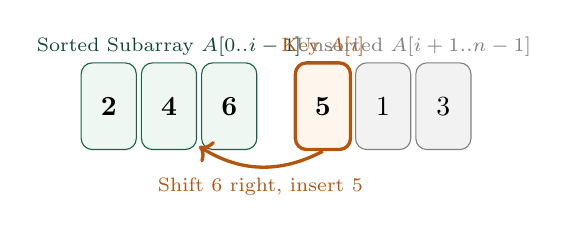
\begin{tikzpicture}[scale=0.85]
  % Sorted hand
  \foreach \x/\v in {0/2, 0.9/4, 1.8/6}{
    \node[draw=ForestGreen, fill=SoftGreen, rounded corners, minimum width=0.7cm, minimum height=1.1cm] at (\x,0) {\textbf{\v}};
  }
  \node[above, DeepGreen, font=\scriptsize] at (0.9, 0.6) {Sorted Subarray $A[0..i-1]$};

  % New incoming card
  \node[draw=DarkOrange, fill=SoftOrange, rounded corners, very thick, minimum width=0.7cm, minimum height=1.1cm] (new) at (3.2,0) {\textbf{5}};
  \node[above, DarkOrange, font=\scriptsize] at (3.2, 0.6) {Key $A[i]$};

  % Unsorted remaining
  \foreach \x/\v in {4.1/1, 5.0/3}{
    \node[draw=gray, fill=black!5, rounded corners, minimum width=0.7cm, minimum height=1.1cm] at (\x,0) {\v};
  }
  \node[above, gray, font=\scriptsize] at (4.55, 0.6) {Unsorted $A[i+1..n-1]$};

  % Shift arrow
  \draw[->, very thick, DarkOrange] (new.south) to[bend left=30] node[below, font=\scriptsize]{Shift 6 right, insert 5} (1.35, -0.6);
\end{tikzpicture}
\end{center}

\subsubsection{Algorithm and Pseudocode}
At step $i$, element `key = A[i]` is compared against elements in the sorted prefix $A[0..i-1]$ from right to left. Elements strictly greater than `key` are shifted one position to the right to create an opening, and `key` is inserted.

\begin{lstlisting}[style=pseudostyle]
FUNCTION INSERTION_SORT(A)
INPUT: array A of length n
OUTPUT: array A sorted in non-decreasing order
    FOR i = 1 TO n - 1 DO
        key = A[i]
        j = i - 1
        WHILE j >= 0 AND A[j] > key DO
            A[j + 1] = A[j]       // Shift element to the right
            j = j - 1
        A[j + 1] = key           // Place key into opening
    RETURN A
\end{lstlisting}

\subsubsection{Step-by-Step Execution Trace}
Consider input array $A = [7, 3, 5, 2, 6, 4]$ ($n = 6$):
\begin{center}
\begin{tabular}{c c l p{7cm}}
\toprule
\textbf{Pass ($i$)} & \textbf{Key ($A[i]$)} & \textbf{Array State After Pass} & \textbf{Internal Shift Operations} \\
\midrule
Start & -- & $[7,\; 3,\; 5,\; 2,\; 6,\; 4]$ & Prefix $A[0..0] = [7]$ is trivially sorted \\
$i = 1$ & $3$ & $[\mathbf{3},\; \mathbf{7},\; 5,\; 2,\; 6,\; 4]$ & $7 > 3 \implies$ 7 shifts right; 3 inserted at index 0 \\
$i = 2$ & $5$ & $[\mathbf{3},\; \mathbf{5},\; \mathbf{7},\; 2,\; 6,\; 4]$ & $7 > 5 \implies$ 7 shifts right; 5 inserted at index 1 \\
$i = 3$ & $2$ & $[\mathbf{2},\; \mathbf{3},\; \mathbf{5},\; \mathbf{7},\; 6,\; 4]$ & $7, 5, 3 > 2 \implies$ all shift right; 2 inserted at index 0 \\
$i = 4$ & $6$ & $[\mathbf{2},\; \mathbf{3},\; \mathbf{5},\; \mathbf{6},\; \mathbf{7},\; 4]$ & $7 > 6 \implies$ 7 shifts right; 6 inserted at index 3 \\
$i = 5$ & $4$ & $[\mathbf{2},\; \mathbf{3},\; \mathbf{4},\; \mathbf{5},\; \mathbf{6},\; \mathbf{7}]$ & $7, 6, 5 > 4 \implies$ shift right; 4 inserted at index 2 \\
\bottomrule
\end{tabular}
\end{center}

\subsubsection{Formal Complexity and Properties}
\begin{itemize}[itemsep=2pt]
    \item \textbf{Loop Invariant:} At the start of each iteration $i$, the subarray $A[0..i-1]$ consists of the original elements in sorted order.
    \item \textbf{Best-Case Time Complexity:} $\Theta(n)$. When the array is already sorted, $A[j] > \text{key}$ evaluates to `False` on the very first comparison for every $i$. The inner loop executes in $O(1)$ time, yielding $T(n) = \sum_{i=1}^{n-1} 1 = n - 1 = \Theta(n)$.
    \item \textbf{Worst-Case Time Complexity:} $\Theta(n^2)$. When the array is reverse sorted, every element must shift past all $i$ predecessors:
    \[
    T_{\text{worst}}(n) = \sum_{i=1}^{n-1} i = \frac{n(n-1)}{2} = \Theta(n^2)
    \]
    \item \textbf{Average-Case Time Complexity:} $\Theta(n^2)$. On average, an element shifts through half of the sorted prefix ($i/2$ comparisons), yielding $\approx n^2/4$ operations.
    \item \textbf{Auxiliary Space:} $\Theta(1)$ (In-place).
    \item \textbf{Stability:} \textbf{Stable.} The condition $A[j] > \text{key}$ uses a strict inequality; when $A[j] == \text{key}$, the while loop terminates, preserving original order.
\end{itemize}

\subsection{Bubble Sort}
\textbf{Conceptual Intuition:} Adjacent pairs of elements are compared sequentially. If out of order, they are swapped. Through repeated sweeps, large elements ``bubble up'' toward the right end of the array, fixing the largest element in place at the end of each pass.

\begin{lstlisting}[style=pseudostyle]
FUNCTION BUBBLE_SORT(A)
INPUT: array A of length n
OUTPUT: array A sorted in non-decreasing order
    FOR end = LENGTH(A) - 1 DOWNTO 1 DO
        swapped = FALSE
        FOR i = 0 TO end - 1 DO
            IF A[i] > A[i + 1] THEN
                SWAP A[i], A[i + 1]
                swapped = TRUE
        IF swapped == FALSE THEN
            RETURN A                    // Early exit if array is already sorted
    RETURN A
\end{lstlisting}

\subsubsection{Step-by-Step Execution Trace with Early Exit}
Trace on array $A = [7, 3, 5, 2, 6, 4]$:
\begin{center}
\begin{tabular}{c c l p{6.5cm}}
\toprule
\textbf{Pass} & \textbf{Fixed Suffix} & \textbf{Array State After Pass} & \textbf{Swaps Performed} \\
\midrule
Start & none & $[7,\; 3,\; 5,\; 2,\; 6,\; 4]$ & Initial state \\
1 & $[7]$ & $[3,\; 5,\; 2,\; 6,\; 4,\; \mathbf{7}]$ & $(7,3), (7,5), (7,2), (7,6), (7,4)$ all swap \\
2 & $[6, 7]$ & $[3,\; 2,\; 5,\; 4,\; \mathbf{6},\; \mathbf{7}]$ & $(5,2), (6,4)$ swap \\
3 & $[5, 6, 7]$ & $[2,\; 3,\; 4,\; \mathbf{5},\; \mathbf{6},\; \mathbf{7}]$ & $(3,2), (5,4)$ swap \\
4 & $[4, 5, 6, 7]$ & $[2,\; 3,\; \mathbf{4},\; \mathbf{5},\; \mathbf{6},\; \mathbf{7}]$ & \textbf{No swaps performed! Early exit triggered.} \\
\bottomrule
\end{tabular}
\end{center}

\subsubsection{Bubble Sort versus Insertion Sort}
Although both have worst-case $O(n^2)$ and best-case $O(n)$ with early termination, \textbf{Insertion Sort is vastly superior in practice}. Bubble Sort requires three memory writes for every adjacent inversion swap (`temp = a; a = b; b = temp`), whereas Insertion Sort shifts elements with a single write (`A[j+1] = A[j]`) and inserts the key only once per outer iteration.

\subsection{Worked Examples and Inversion Analysis for Elementary Sorts}

\begin{examplebox}[Example 2.1 (Predicting Work on Partially Sorted Data)]
Consider running Insertion Sort and Bubble Sort on three arrays of size $n = 6$:
\begin{enumerate}[itemsep=2pt]
    \item \textbf{Case A (Already Sorted):} $A_1 = [2, 3, 4, 5, 6, 7]$.
    \begin{itemize}[itemsep=1pt]
        \item \emph{Insertion Sort:} Each $A[i]$ immediately satisfies $A[i-1] \le A[i]$. Only $n - 1 = 5$ comparisons and $0$ shifts occur. Total time: $\Theta(n)$.
        \item \emph{Bubble Sort (Optimized):} Pass 1 compares all 5 adjacent pairs. No swaps occur; `swapped` remains `False`. The algorithm terminates after 5 comparisons and 0 swaps. Total time: $\Theta(n)$.
    \end{itemize}
    \item \textbf{Case B (Single Misplaced Item at Front):} $A_2 = [7, 2, 3, 4, 5, 6]$.
    \begin{itemize}[itemsep=1pt]
        \item \emph{Insertion Sort:} For $i=1$, element $2$ shifts past $7$. For all subsequent $i \ge 2$, elements are already in order. Total comparisons: $1 + 1 + 1 + 1 + 1 = 5$. Total shifts: $1$. Total time: $O(n)$.
        \item \emph{Bubble Sort:} Value $7$ must bubble across the entire array in Pass 1 (5 swaps). Pass 2 checks all remaining pairs (no swaps) and terminates. Total comparisons: $5 + 4 = 9$, total swaps: $5$.
    \end{itemize}
    \item \textbf{Case C (Strictly Reverse-Sorted):} $A_3 = [7, 6, 5, 4, 3, 2]$.
    \begin{itemize}[itemsep=1pt]
        \item \emph{Insertion Sort:} Maximum possible shifts. Total comparisons and shifts: $\sum_{i=1}^5 i = 15$. Total time: $\Theta(n^2)$.
        \item \emph{Bubble Sort:} Maximum possible passes ($n-1 = 5$). Total comparisons: $5 + 4 + 3 + 2 + 1 = 15$, total swaps: $15$.
    \end{itemize}
\end{enumerate}
\end{examplebox}

\begin{theorembox}[Theorem 2.1 (Inversion Count Connection)]
An \textbf{inversion} in an array $A$ is a pair of indices $(i, j)$ such that $i < j$ and $A[i] > A[j]$. If an array contains $I$ inversions:
\begin{itemize}[itemsep=1pt]
    \item Every adjacent swap in Bubble Sort or shift in Insertion Sort eliminates exactly \textbf{one} inversion.
    \item The running time of Insertion Sort is strictly $\Theta(n + I)$.
    \item When an array is ``nearly sorted'' such that $I = O(n)$, Insertion Sort runs in strictly linear $\Theta(n)$ time.
\end{itemize}
\end{theorembox}

\newpage
% =========================================================================
\section{Efficient Divide-and-Conquer Sorts: Merge Sort and Quick Sort}
% =========================================================================

\subsection{Merge Sort}
Merge Sort applies the classic \textbf{Divide-and-Conquer} paradigm:
\begin{enumerate}[itemsep=1pt]
    \item \textbf{Divide:} Partition array of size $n$ into two equal sublists of size $\lfloor n/2 \rfloor$ and $\lceil n/2 \rceil$.
    \item \textbf{Conquer:} Recursively sort each sublist. Base case: a list of size $\le 1$ is already sorted.
    \item \textbf{Combine:} Merge the two sorted sublists into a single sorted array.
\end{enumerate}

\begin{center}
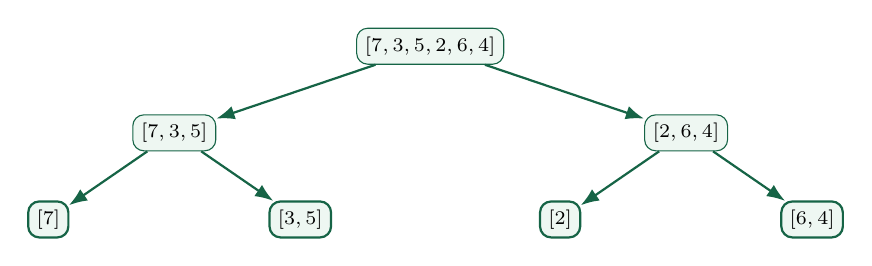
\begin{tikzpicture}[
    level 1/.style={sibling distance=6.5cm, level distance=1.1cm},
    level 2/.style={sibling distance=3.2cm, level distance=1.1cm},
    every node/.style={draw=ForestGreen, fill=SoftGreen, rounded corners, font=\scriptsize\bfseries, inner sep=3pt},
    edge from parent/.style={draw=ForestGreen, -Latex, thick}
]
\node {$[7, 3, 5, 2, 6, 4]$}
    child { node {$[7, 3, 5]$}
        child { node {$[7]$} }
        child { node {$[3, 5]$} }
    }
    child { node {$[2, 6, 4]$}
        child { node {$[2]$} }
        child { node {$[6, 4]$} }
    };
\end{tikzpicture}
\end{center}

\subsubsection{Formal Merge and Merge Sort Pseudocode}
\begin{lstlisting}[style=pseudostyle]
FUNCTION MERGE(L, R)
INPUT: sorted arrays L and R
OUTPUT: one combined sorted array containing all values
    result = empty array
    i = 0; j = 0
    WHILE i < LENGTH(L) AND j < LENGTH(R) DO
        IF L[i] <= R[j] THEN             // <= ensures STABILITY
            APPEND L[i] TO result; i = i + 1
        ELSE
            APPEND R[j] TO result; j = j + 1
    APPEND all remaining elements of L TO result
    APPEND all remaining elements of R TO result
    RETURN result

FUNCTION MERGE_SORT(A)
INPUT: array A
OUTPUT: sorted array
    IF LENGTH(A) <= 1 THEN RETURN A
    mid = LENGTH(A) DIV 2
    L = MERGE_SORT(A[0 : mid])
    R = MERGE_SORT(A[mid : LENGTH(A)])
    RETURN MERGE(L, R)
\end{lstlisting}

\subsubsection{Mathematical Complexity Analysis}
The recurrence relation for Merge Sort on an input of size $n$ is:
\[
T(n) = 2 T\left(\frac{n}{2}\right) + \Theta(n)
\]
Using the Master Theorem: $a = 2, b = 2, f(n) = \Theta(n)$. The watershed function is $n^{\log_b a} = n^{\log_2 2} = n^1$. Since $f(n) = \Theta(n^1)$, this falls into \textbf{Case 2}:
\[
T(n) = \Theta(n \log n) \quad \text{in Best, Average, and Worst Cases!}
\]
\textbf{Tradeoffs:}
\begin{itemize}[itemsep=2pt]
    \item \textbf{Advantage:} Predictable $\Theta(n \log n)$ guarantee; completely immune to bad inputs; \textbf{stable}.
    \item \textbf{Disadvantage:} \textbf{Not in-place}. Merging requires $\Theta(n)$ auxiliary buffer space.
\end{itemize}

\subsection{Quick Sort}
Quick Sort operates by choosing an element called a \textbf{pivot}, partitioning the remaining elements into two groups—those less than or equal to the pivot, and those greater than the pivot—and then recursively sorting each group.

\subsubsection{Lomuto Partition Scheme and Quicksort Pseudocode}
\begin{lstlisting}[style=pseudostyle]
FUNCTION QUICK_SORT(A, low, high)
    IF low >= high THEN RETURN
    p = PARTITION(A, low, high)
    QUICK_SORT(A, low, p - 1)
    QUICK_SORT(A, p + 1, high)

FUNCTION PARTITION(A, low, high)
    pivot = A[high]                 // Choose last element as pivot
    boundary = low
    FOR scan = low TO high - 1 DO
        IF A[scan] <= pivot THEN
            SWAP A[boundary], A[scan]
            boundary = boundary + 1
    SWAP A[boundary], A[high]        // Put pivot into correct final slot
    RETURN boundary
\end{lstlisting}

\subsubsection{Trace of Lomuto Partitioning}
Trace on subarray $[7, 3, 5, 2, 6, 4]$ with pivot $= 4$:
\begin{center}
\begin{tabular}{c c l p{6.5cm}}
\toprule
\textbf{Scan Index} & \textbf{Scanned Value} & \textbf{Action Taken} & \textbf{Array State ($boundary$ position)} \\
\midrule
Start & -- & pivot $= 4$ & $[7,\; 3,\; 5,\; 2,\; 6,\; \mathbf{4}]$, $boundary = 0$ \\
$scan = 0$ & $7$ & $7 > 4 \implies$ do nothing & $[7,\; 3,\; 5,\; 2,\; 6,\; \mathbf{4}]$, $boundary = 0$ \\
$scan = 1$ & $3$ & $3 \le 4 \implies$ swap with $A[0]$ & $[3,\; 7,\; 5,\; 2,\; 6,\; \mathbf{4}]$, $boundary = 1$ \\
$scan = 2$ & $5$ & $5 > 4 \implies$ do nothing & $[3,\; 7,\; 5,\; 2,\; 6,\; \mathbf{4}]$, $boundary = 1$ \\
$scan = 3$ & $2$ & $2 \le 4 \implies$ swap with $A[1]$ & $[3,\; 2,\; 5,\; 7,\; 6,\; \mathbf{4}]$, $boundary = 2$ \\
$scan = 4$ & $6$ & $6 > 4 \implies$ do nothing & $[3,\; 2,\; 5,\; 7,\; 6,\; \mathbf{4}]$, $boundary = 2$ \\
Finish & -- & Swap $A[2]$ with pivot $A[5]$ & $[\mathbf{3},\; \mathbf{2},\; \mathbf{4},\; \mathbf{7},\; \mathbf{6},\; \mathbf{5}]$, return $boundary = 2$ \\
\bottomrule
\end{tabular}
\end{center}

\subsubsection{The Pivotal Role of Pivot Selection}
\begin{itemize}[itemsep=2pt]
    \item \textbf{Best Case (Balanced Split):} Pivot is always the median. $T(n) = 2T(n/2) + \Theta(n) \implies \Theta(n \log n)$.
    \item \textbf{Worst Case (Degenerate Split):} Naive pivot on already sorted array. Partition produces subproblems of size $0$ and $n-1$:
    \[
    T(n) = T(n - 1) + \Theta(n) = \sum_{i=1}^n i = \Theta(n^2)
    \]
    \item \textbf{Average Case:} $T(n) = \Theta(n \log n)$ with small constant factors.
    \item \textbf{Solutions to Worst-Case:} (1) \textbf{Randomized Quicksort} (swap random index with `high` before partitioning), (2) \textbf{Median-of-Three} (take median of $\{A[low], A[mid], A[high]\}$).
    \item \textbf{Stability:} \textbf{Unstable} due to long-distance swaps during partitioning.
\end{itemize}

\subsection{Worked Examples on Divide-and-Conquer Sorting}

\begin{examplebox}[Example 3.1 (Tracing the Two-Way Merge Step-by-Step)]
Suppose the recursive calls have sorted two halves into $L = [3, 5, 7]$ and $R = [2, 4, 6]$. The `MERGE(L, R)` function combines them into a single sorted array by maintaining pointers $i$ and $j$:
\begin{center}
\begin{tabular}{c c c c l}
\toprule
\textbf{Step} & \textbf{Compare $L[i]$ vs $R[j]$} & \textbf{Condition} & \textbf{Selected Item} & \textbf{Output Array So Far} \\
\midrule
1 & $L[0]=3$ vs $R[0]=2$ & $3 > 2$ & $R[0]=2$, advance $j \to 1$ & $[2]$ \\
2 & $L[0]=3$ vs $R[1]=4$ & $3 \le 4$ & $L[0]=3$, advance $i \to 1$ & $[2, 3]$ \\
3 & $L[1]=5$ vs $R[1]=4$ & $5 > 4$ & $R[1]=4$, advance $j \to 2$ & $[2, 3, 4]$ \\
4 & $L[1]=5$ vs $R[2]=6$ & $5 \le 6$ & $L[1]=5$, advance $i \to 2$ & $[2, 3, 4, 5]$ \\
5 & $L[2]=7$ vs $R[2]=6$ & $7 > 6$ & $R[2]=6$, advance $j \to 3$ & $[2, 3, 4, 5, 6]$ \\
6 & $R$ is exhausted & -- & Append remaining $L[2]=7$ & $[2, 3, 4, 5, 6, 7]$ \\
\bottomrule
\end{tabular}
\end{center}
\textbf{Key Observation:} Exactly 5 comparisons were needed to merge $3 + 3 = 6$ elements. In general, merging lists of size $n_1$ and $n_2$ requires at most $n_1 + n_2 - 1$ comparisons, proving the merge step is strictly $\Theta(n)$.
\end{examplebox}

\begin{examplebox}[Example 3.2 (Quicksort Degeneracy: Naive vs Median-of-Three Pivot)]
Consider sorting the already sorted sequence $A = [1, 2, 3, 4, 5]$:
\begin{itemize}[itemsep=2pt]
    \item \textbf{Naive Strategy (Last Element as Pivot):}
    \begin{itemize}[itemsep=1pt]
        \item Call 1: Pivot $= 5$. Partition splits into $[1, 2, 3, 4]$ (left) and $[]$ (right). Comparisons: 4.
        \item Call 2: Pivot $= 4$. Partition splits into $[1, 2, 3]$ (left) and $[]$ (right). Comparisons: 3.
        \item Call 3: Pivot $= 3$. Partition splits into $[1, 2]$ and $[]$. Comparisons: 2.
        \item Call 4: Pivot $= 2$. Partition splits into $[1]$ and $[]$. Comparisons: 1.
        \item \textbf{Recursion Tree:} Completely skewed chain of depth $n-1 = 4$. Total comparisons: $4 + 3 + 2 + 1 = 10 = \frac{n(n-1)}{2} = \Theta(n^2)$.
    \end{itemize}
    \item \textbf{Median-of-Three Strategy:}
    Sample $\{A[0]=1, A[2]=3, A[4]=5\}$. The median is $3$. Swapping $3$ to the end as pivot splits the array into $[1, 2]$ and $[4, 5]$: two perfectly balanced halves! The tree height is $\lceil \log_2 5 \rceil = 3$, and total comparisons are bounded by $O(n \log n)$.
\end{itemize}
\end{examplebox}

\newpage
% =========================================================================
\section{Non-Comparison Linear-Time Sorting: Counting Sort \& Radix Sort}
% =========================================================================

\subsection{The \texorpdfstring{$\Omega(n \log n)$}{Omega(n log n)} Lower Bound for Comparison Sorts}

\begin{theorembox}[Theorem 4.1 (Information-Theoretic Lower Bound)]
Any comparison-based sorting algorithm requires at least $\Omega(n \log n)$ comparisons in the worst case to sort $n$ distinct elements.
\end{theorembox}
\textbf{Proof via Decision Trees:}
\begin{enumerate}[itemsep=2pt]
    \item Any comparison sort can be modeled as a binary decision tree where each internal node represents a comparison $A[i] \le A[j]$ and each leaf represents a distinct sorted permutation of the input.
    \item An array of $n$ elements has $n!$ possible permutations. The decision tree must contain at least $n!$ reachable leaves ($L \ge n!$).
    \item A binary tree of height $h$ can have at most $2^h$ leaves. Therefore:
    \[
    2^h \ge L \ge n! \implies h \ge \log_2(n!)
    \]
    \item Applying Stirling's approximation ($\ln(n!) = n \ln n - n + O(\ln n)$):
    \[
    h \ge \log_2(n!) = \sum_{i=1}^n \log_2 i \ge \sum_{i=n/2}^n \log_2(n/2) = \frac{n}{2} (\log_2 n - 1) = \Omega(n \log n)
    \]
\end{enumerate}
To achieve linear $O(n)$ sorting time, an algorithm must be \textbf{non-comparison-based}, leveraging integer keys as indices.

\subsection{Counting Sort}
Counting Sort assumes all $n$ input keys are non-negative integers bounded by a known integer $k$ (i.e., keys $\in \{0, 1, \dots, k\}$).

\begin{lstlisting}[style=pseudostyle]
FUNCTION COUNTING_SORT(A, k)
INPUT: array A of n integer keys in {0, ..., k}
OUTPUT: stable sorted array B
    CREATE count[0 .. k] initialized to 0
    FOR i = 0 TO n - 1 DO                   // Pass 1: Frequency histogram
        count[A[i]] = count[A[i]] + 1
    FOR key = 1 TO k DO                     // Pass 2: Prefix sums (positions)
        count[key] = count[key] + count[key - 1]
    CREATE output array B of length n
    FOR i = n - 1 DOWNTO 0 DO               // Pass 3: Backwards placement (STABILITY)
        key = A[i]
        B[count[key] - 1] = A[i]
        count[key] = count[key] - 1
    RETURN B
\end{lstlisting}

\subsubsection{Why Counting Sort Must Scan Backwards for Stability}
In Pass 3, traversing $i$ from $n-1$ down to $0$ ensures that when duplicate keys are encountered, the one appearing later in the input array receives the highest available precomputed position (`count[key] - 1`), thus preserving the initial relative ordering.

\subsubsection{Complexity Analysis and Constraints}
\begin{itemize}[itemsep=2pt]
    \item \textbf{Time Complexity:} $\Theta(n + k)$. Allocating and zeroing `count` takes $\Theta(k)$; Pass 1 takes $\Theta(n)$; Pass 2 takes $\Theta(k)$; Pass 3 takes $\Theta(n)$.
    \item \textbf{When is it Linear?} If $k = O(n)$, then $T(n) = \Theta(n + n) = \Theta(n)$.
    \item \textbf{When does it fail?} If $n = 10$ and keys are in range $0$ to $1,000,000,000$, Counting Sort allocates an array of 1 billion elements, requiring gigabytes of RAM and billions of operations!
\end{itemize}

\subsection{Radix Sort}
Radix Sort resolves Counting Sort's memory limitation by sorting multi-digit numbers digit by digit, from \textbf{Least Significant Digit (LSD)} to Most Significant Digit (MSD).

\begin{lstlisting}[style=pseudostyle]
FUNCTION RADIX_SORT(A, d, b)
INPUT: array A of n non-negative integers with at most d digits in base b
OUTPUT: array A sorted in non-decreasing order
    FOR digit_pos = 0 TO d - 1 DO
        A = STABLE_COUNTING_SORT_BY_DIGIT(A, digit_pos, b)
    RETURN A
\end{lstlisting}

\begin{theorembox}[Theorem 4.2 (Radix Sort Correctness and Complexity)]
If the underlying digit-sort subroutine is \textbf{stable}, Radix Sort correctly sorts numbers with $d$ digits in base $b$ in $\Theta(d(n + b))$ time using $\Theta(n + b)$ auxiliary space.
\end{theorembox}
\textbf{Example:} To sort 32-bit integers, we can choose base $b = 2^8 = 256$ (1 byte). Any 32-bit integer has $d = 4$ bytes. Radix sort requires exactly $d = 4$ stable counting passes, each with $k = 256$, sorting $n$ records in $\Theta(4(n + 256)) = \Theta(n)$ time!

\subsection{Worked Examples: Counting Sort and Radix Sort Traces}

\begin{examplebox}[Example 4.1 (Full Step-by-Step Counting Sort Trace)]
Consider sorting the array $A = [2, 5, 3, 0, 2, 3, 0, 3]$ with $n = 8$ and maximum key $k = 5$:
\begin{enumerate}[itemsep=2pt]
    \item \textbf{Pass 1 (Frequency Counting):} Initialize `count[0..5] = [0, 0, 0, 0, 0, 0]`. After scanning $A$:
    \[
    \text{count} = [2,\; 0,\; 2,\; 3,\; 0,\; 1] \quad (\text{two } 0\text{s, zero } 1\text{s, two } 2\text{s, three } 3\text{s, zero } 4\text{s, one } 5)
    \]
    \item \textbf{Pass 2 (Prefix Sums):} Accumulate running totals to determine ending positions:
    \[
    \text{count}[0]=2,\; \text{count}[1]=2,\; \text{count}[2]=4,\; \text{count}[3]=7,\; \text{count}[4]=7,\; \text{count}[5]=8
    \]
    \item \textbf{Pass 3 (Backwards Placement into $B[0..7]$):}
    \begin{center}
    \begin{tabular}{c c c c l}
    \toprule
    \textbf{Step} & \textbf{Item $A[i]$} & \textbf{Target Index `count[key]-1`} & \textbf{Decrement Count} & \textbf{Array $B$ State} \\
    \midrule
    $i = 7$ & $A[7] = 3$ & index $7 - 1 = 6$ & `count[3]` becomes 6 & $[\_,\; \_,\; \_,\; \_,\; \_,\; \_, \mathbf{3},\; \_]$ \\
    $i = 6$ & $A[6] = 0$ & index $2 - 1 = 1$ & `count[0]` becomes 1 & $[\_,\; \mathbf{0},\; \_,\; \_,\; \_,\; \_, 3,\; \_]$ \\
    $i = 5$ & $A[5] = 3$ & index $6 - 1 = 5$ & `count[3]` becomes 5 & $[\_,\; 0,\; \_,\; \_,\; \_,\; \mathbf{3},\; 3,\; \_]$ \\
    $i = 4$ & $A[4] = 2$ & index $4 - 1 = 3$ & `count[2]` becomes 3 & $[\_,\; 0,\; \_,\; \mathbf{2},\; \_,\; 3,\; 3,\; \_]$ \\
    $i = 3$ & $A[3] = 0$ & index $1 - 1 = 0$ & `count[0]` becomes 0 & $[\mathbf{0},\; 0,\; \_,\; 2,\; \_,\; 3,\; 3,\; \_]$ \\
    $i = 2$ & $A[2] = 3$ & index $5 - 1 = 4$ & `count[3]` becomes 4 & $[0,\; 0,\; \_,\; 2,\; \mathbf{3},\; 3,\; 3,\; \_]$ \\
    $i = 1$ & $A[1] = 5$ & index $8 - 1 = 7$ & `count[5]` becomes 7 & $[0,\; 0,\; \_,\; 2,\; 3,\; 3,\; 3,\; \mathbf{5}]$ \\
    $i = 0$ & $A[0] = 2$ & index $3 - 1 = 2$ & `count[2]` becomes 2 & $[0,\; 0,\; \mathbf{2},\; 2,\; 3,\; 3,\; 3,\; 5]$ \\
    \bottomrule
    \end{tabular}
    \end{center}
    Notice how the three occurrences of $3$ preserve their relative arrival order in slots 4, 5, and 6, proving stability!
\end{enumerate}
\end{examplebox}

\begin{examplebox}[Example 4.2 (Full Step-by-Step Radix Sort Trace)]
Sort the list of 3-digit decimal integers $A = [170, 045, 075, 090, 802, 024, 002, 066]$ ($n = 8, d = 3, b = 10$):
\begin{itemize}[itemsep=3pt]
    \item \textbf{Pass 1 (Sort stably by least significant digit -- units place $10^0$):}\\
    Comparing digits $[\underline{0}, \underline{5}, \underline{5}, \underline{0}, \underline{2}, \underline{4}, \underline{2}, \underline{6}]$:\\
    Result $A^{(1)} = [17\mathbf{0},\; 09\mathbf{0},\; 80\mathbf{2},\; 00\mathbf{2},\; 02\mathbf{4},\; 04\mathbf{5},\; 07\mathbf{5},\; 06\mathbf{6}]$
    \item \textbf{Pass 2 (Sort stably by middle digit -- tens place $10^1$):}\\
    Comparing digits $[\underline{7}, \underline{9}, \underline{0}, \underline{0}, \underline{2}, \underline{4}, \underline{7}, \underline{6}]$ on $A^{(1)}$:\\
    Result $A^{(2)} = [8\mathbf{0}2,\; 0\mathbf{0}2,\; 0\mathbf{2}4,\; 0\mathbf{4}5,\; 0\mathbf{6}6,\; 1\mathbf{7}0,\; 0\mathbf{7}5,\; 0\mathbf{9}0]$ \quad (\emph{Notice $802$ precedes $002$ because $802$ preceded $002$ in $A^{(1)}$!})
    \item \textbf{Pass 3 (Sort stably by most significant digit -- hundreds place $10^2$):}\\
    Comparing digits $[\underline{8}, \underline{0}, \underline{0}, \underline{0}, \underline{0}, \underline{1}, \underline{0}, \underline{0}]$ on $A^{(2)}$:\\
    Final Sorted Result $A^{(3)} = [\mathbf{0}02,\; \mathbf{0}24,\; \mathbf{0}45,\; \mathbf{0}66,\; \mathbf{0}75,\; \mathbf{0}90,\; \mathbf{1}70,\; \mathbf{8}02]$
\end{itemize}
All elements are now completely sorted in exactly 3 passes of 8 elements each!
\end{examplebox}

\newpage
% =========================================================================
\section{Python Sorting in Practice}
% =========================================================================

\subsection{Python's Built-in Sorting: `sorted()` vs. `list.sort()`}
Python incorporates \textbf{Timsort} (engineered by Tim Peters in 2002), an adaptive hybrid of Merge Sort and Insertion Sort:
\begin{itemize}[itemsep=2pt]
    \item Finds naturally occurring ordered sequences (``runs'') in $O(n)$ time.
    \item Uses binary insertion sort on short runs and merges balanced runs with an intelligent stack mechanism.
    \item Guarantees $\Theta(n \log n)$ worst-case, $\Theta(n)$ best-case on presorted data, and is strictly \textbf{stable}.
\end{itemize}

\begin{lstlisting}[style=pythonstyle]
# sorted() returns a NEW sorted list (works on any iterable, original unchanged)
original = [7, 3, 5, 2]
new_list = sorted(original)         # original remains [7, 3, 5, 2]

# list.sort() sorts the list IN-PLACE and returns None
original.sort()                     # original is now [2, 3, 5, 7]
\end{lstlisting}

\subsubsection{Multi-Attribute Sorting with Keys}
Python's `key` parameter accepts a callable that extracts a comparison key from each element before sorting:
\begin{lstlisting}[style=pythonstyle]
students = [
    {"id": "S1", "name": "Lan", "gpa": 3.4},
    {"id": "S2", "name": "Minh", "gpa": 3.8},
    {"id": "S3", "name": "An", "gpa": 3.8},
]

# Sort by GPA descending (-gpa), then by Name ascending (s["name"])
ranked = sorted(students, key=lambda s: (-s["gpa"], s["name"]))
# Result: S3 (An, 3.8), S2 (Minh, 3.8), S1 (Lan, 3.4)
\end{lstlisting}

\subsection{Practical Python Sorting Case Studies}

\begin{examplebox}[Example 5.1 (Multi-Criteria Product Catalog Sorting)]
Suppose an online retail backend receives products with multiple attributes and needs to sort by \textbf{Category} ascending, then by \textbf{Rating} descending, and finally by \textbf{Price} ascending. Because Python evaluates tuples lexicographically element-by-element, a tuple-based \lstinline{key} resolves all primary, secondary, and tertiary criteria in a single $O(n \log n)$ pass.
\end{examplebox}

\begin{lstlisting}[style=pythonstyle]
products = [
    {"name": "Laptop Pro", "category": "Electronics", "rating": 4.8, "price": 1200},
    {"name": "Gaming PC",   "category": "Electronics", "rating": 4.9, "price": 1800},
    {"name": "Notebook",    "category": "Books",       "rating": 4.8, "price": 15},
    {"name": "Desk Lamp",   "category": "Electronics", "rating": 4.8, "price": 45},
]

# Sort by Category ascending, then by Rating descending, then by Price ascending
sorted_products = sorted(
    products,
    key=lambda p: (p["category"], -p["rating"], p["price"])
)
\end{lstlisting}

\begin{examplebox}[Example 5.2 (Emulating Custom Comparison Functions)]
When sorting complex geometries, intervals, or custom objects where a single-value key projection is cumbersome, we can use \lstinline{functools.cmp_to_key} to adapt a two-argument comparator $(a, b)$ to modern Python's key-based interface:
\end{examplebox}

\begin{lstlisting}[style=pythonstyle]
from functools import cmp_to_key

# Sort intervals [start, end]: earlier start first; if tie, longer interval first
intervals = [(1, 4), (2, 6), (1, 8), (3, 5)]

def compare_intervals(a, b):
    if a[0] != b[0]:
        return -1 if a[0] < b[0] else 1
    # Tie in start: larger end comes first (descending)
    return -1 if a[1] > b[1] else (1 if a[1] < b[1] else 0)

sorted_intervals = sorted(intervals, key=cmp_to_key(compare_intervals))
# Result: [(1, 8), (1, 4), (2, 6), (3, 5)]
\end{lstlisting}

\subsection{Common Sorting Mistakes and Anti-Patterns}
\begin{notebox}[Common Traps in Sorting]
\begin{enumerate}[itemsep=2pt]
    \item \textbf{Assigning the result of `list.sort()`:} Writing `x = x.sort()` sets `x = None` because `sort()` modifies in place and returns `None`!
    \item \textbf{Assuming Quicksort is always fast:} Using naive Quicksort on sorted data produces $O(n^2)$ time and call-stack crashes (`RecursionError`).
    \item \textbf{Using Counting Sort on floating-point or large ranges:} Counting sort requires non-negative integers; using it for floats or $10^9$ ranges causes out-of-memory errors.
    \item \textbf{Breaking Stability Unintentionally:} In Merge Sort or Counting Sort, replacing `<=` with `<` destroys stability.
\end{enumerate}
\end{notebox}

\newpage
% =========================================================================
\section{The Selection Problem and Order Statistics}
% =========================================================================

\subsection{Order Statistics and Ranks}
\begin{definitionbox}[Definition 6.1 (The Selection Problem)]
Given a collection of $n$ elements $A$ and an integer $k \in \{1, 2, \dots, n\}$, find the element that would occupy index $k - 1$ if the array were sorted in non-decreasing order. This element is called the \textbf{$k$-th order statistic} (or element of rank $k$).
\begin{itemize}[itemsep=1pt]
    \item Rank $k = 1$: Minimum value.
    \item Rank $k = n$: Maximum value.
    \item Rank $k = \lceil n/2 \rceil$: Median.
\end{itemize}
\end{definitionbox}

\subsection{Finding Extremes in a Single Scan: \texorpdfstring{$\Theta(n)$}{Theta(n)}}
Finding the minimum or maximum requires only $n - 1$ comparisons:
\begin{lstlisting}[style=pseudostyle]
FUNCTION MINIMUM(A)
INPUT: non-empty array A
OUTPUT: smallest value in A
    best = A[0]
    FOR i = 1 TO LENGTH(A) - 1 DO
        IF A[i] < best THEN best = A[i]
    RETURN best
\end{lstlisting}
\textbf{Note:} Finding \emph{both} the minimum and maximum simultaneously can be achieved in $\lceil 3n/2 \rceil - 2$ comparisons (rather than $2n - 2$) by processing elements in pairs and comparing the larger against current max and smaller against current min.

\subsection{Strategies for General Rank Selection}
\begin{center}
\begin{tabularx}{\textwidth}{p{3.5cm} c p{7.5cm}}
\toprule
\textbf{Strategy} & \textbf{Time Complexity} & \textbf{Practical Assessment} \\
\midrule
\textbf{Sort, then index} & $\Theta(n \log n)$ & Ideal if multiple rank queries follow or full sorted output is required. \\
\textbf{Repeated selection} & $\Theta(k \cdot n)$ & Viable only for very small $k$ ($k \le 3$). Inefficient for medians ($k = n/2$). \\
\textbf{Quickselect} & Expected $\Theta(n)$ & Optimal in-place choice for a single rank query on an in-memory array. \\
\textbf{Heap of size $k$} & $\Theta(n \log k)$ & Optimal for finding Top-$k$ items in a live continuous data stream. \\
\textbf{Median of Medians} & Worst-case $\Theta(n)$ & Theoretical breakthrough ensuring $O(n)$ worst-case pivot selection. \\
\bottomrule
\end{tabularx}
\end{center}

\subsection{Quickselect (Hoare's Selection Algorithm)}
Quickselect exploits the fact that the partition subroutine of Quicksort places the chosen pivot into its final sorted position $p$. If $p$ matches our target rank, we are done; otherwise, we recurse \textbf{into only one partition}, discarding the other!

\begin{lstlisting}[style=pseudostyle]
FUNCTION QUICKSELECT(A, k)
INPUT: array A, rank k (1 <= k <= LENGTH(A))
OUTPUT: the kth-smallest value in A
    target = k - 1                          // Convert 1-based rank to 0-based index
    low = 0; high = LENGTH(A) - 1
    WHILE low <= high DO
        p = PARTITION(A, low, high)         // Same partition as Quicksort
        IF p == target THEN
            RETURN A[p]                     // Target found!
        ELSE IF target < p THEN
            high = p - 1                    // Target is in left partition
        ELSE
            low = p + 1                     // Target is in right partition
\end{lstlisting}

\subsubsection{Trace for 5th-Smallest Value \texorpdfstring{($k = 5 \implies \text{target index } 4$)}{(k = 5)}}
Trace on $A = [7, 3, 5, 2, 6, 4]$:
\begin{center}
\begin{tabularx}{\textwidth}{c c c X}
\toprule
\textbf{Active Range} & \textbf{Array State} & \textbf{Pivot Index $p$} & \textbf{Action} \\
\midrule
$[0..5]$ & $[3, 2, \mathbf{4}, 7, 6, 5]$ & $p = 2$ (value $4$) & $4 < \text{target } 4 \implies low = 3$ (Search right $[7, 6, 5]$) \\
$[3..5]$ & $[3, 2, 4, \mathbf{5}, 6, 7]$ & $p = 3$ (value $5$) & $5 < \text{target } 4 \implies low = 4$ (Search right $[6, 7]$) \\
$[4..5]$ & $[3, 2, 4, 5, \mathbf{6}, 7]$ & $p = 4$ (value $6$) & $p == \text{target } 4 \implies \textbf{Return } 6$! \\
\bottomrule
\end{tabularx}
\end{center}

\subsubsection{Quickselect Complexity Analysis}
\begin{itemize}[itemsep=2pt]
    \item \textbf{Average Case:} On each step, array size halves: $n + \frac{n}{2} + \frac{n}{4} + \dots \le 2n = \Theta(n)$.
    \item \textbf{Worst Case:} Naive pivot splits $0$ and $n-1$: $n + (n-1) + \dots + 1 = \Theta(n^2)$.
\end{itemize}

\subsection{The Median of Medians Algorithm (BFPRT)}
Invented by Blum, Floyd, Pratt, Rivest, and Tarjan (1973), this algorithm guarantees a good pivot deterministically:
\begin{enumerate}[itemsep=1pt]
    \item Divide $n$ elements into $\lfloor n/5 \rfloor$ groups of 5 elements (and one remainder group).
    \item Find the median of each group of 5 using insertion sort ($O(1)$ per group, $O(n)$ total).
    \item Recursively find the median of the $\lceil n/5 \rceil$ medians; call this pivot $x$.
    \item Partition array around $x$. At least $30\%$ of elements are strictly smaller than $x$ and at least $30\%$ are strictly larger! The remaining subproblem is guaranteed to be at most $\frac{7}{10}n$.
\end{enumerate}
\textbf{Recurrence Relation:}
\[
T(n) \le T\left(\frac{n}{5}\right) + T\left(\frac{7n}{10}\right) + \Theta(n)
\]
Because $\frac{1}{5} + \frac{7}{10} = \frac{9}{10} < 1$, the sum of subproblem fractions is strictly less than 1. By induction/substitution, $T(n) = \Theta(n)$ \textbf{in the absolute worst case}.

\subsection{Worked Examples in Selection and Top-\texorpdfstring{$k$}{k} Extraction}

\begin{examplebox}[Example 6.1 (Finding the Median of 7 Numbers with Quickselect)]
Find the median (rank $k = 4 \implies \text{target index } 3$) of the unsorted array $A = [9, 4, 8, 2, 7, 1, 5]$ ($n = 7$):
\begin{enumerate}[itemsep=2pt]
    \item \textbf{Call 1 (Range $low = 0, high = 6$):} Pivot $A[6] = 5$.
    \begin{itemize}[itemsep=1pt]
        \item Elements $\le 5$: $4, 2, 1$. Elements $> 5$: $9, 8, 7$.
        \item After partition: Array becomes $[4, 2, 1, \mathbf{5}, 7, 9, 8]$ with pivot index $p = 3$.
        \item Pivot index $p = 3$ matches our target index $3$ on the very first try!
        \item \textbf{Result:} Median is $5$. Total comparisons: 6.
    \end{itemize}
\end{enumerate}
\end{examplebox}

\begin{examplebox}[Example 6.2 (Streaming Top-$k$ Processing via Python \lstinline{heapq})]
When extracting the top $k = 3$ largest transactions from a continuous streaming log of millions of records, keeping all records in memory is prohibited. Instead, maintain a min-heap of size $k=3$. For $n$ stream elements, memory usage is strictly $O(k)$, and total runtime is $O(n \log k)$. For $k \ll n$, this is practically linear!
\end{examplebox}

\begin{lstlisting}[style=pythonstyle]
import heapq

def top_k_streaming(stream, k):
    # Initialize heap with the first k elements
    min_heap = []
    for value in stream:
        if len(min_heap) < k:
            heapq.heappush(min_heap, value)
        elif value > min_heap[0]:
            # If current value exceeds the smallest in top-k, replace it
            heapq.heappushpop(min_heap, value)
    return sorted(min_heap, reverse=True)

# Example usage on incoming scores
scores = [12, 85, 45, 92, 60, 99, 74, 30]
print(top_k_streaming(scores, 3))   # Output: [99, 92, 85]
\end{lstlisting}

\newpage
% =========================================================================
\section{Searching Algorithms: Linear, Binary, and Ternary Search}
% =========================================================================

\subsection{Linear Search}
For unsorted collections, we inspect elements sequentially from left to right:
\begin{lstlisting}[style=pseudostyle]
FUNCTION LINEAR_SEARCH(A, target)
    FOR i = 0 TO LENGTH(A) - 1 DO
        IF A[i] == target THEN RETURN i
    RETURN NONE
\end{lstlisting}
\textbf{Complexity:} Best case $\Omega(1)$ (target at index 0); Worst case $O(n)$ (target absent); Average case $\frac{n+1}{2} = \Theta(n)$.

\subsection{Binary Search}
\textbf{Prerequisite:} The collection $A$ \textbf{must be sorted} in non-decreasing order.

\begin{lstlisting}[style=pseudostyle]
FUNCTION BINARY_SEARCH(A, target)
INPUT: sorted array A, search target
OUTPUT: index of target, or NONE
    low = 0
    high = LENGTH(A) - 1
    WHILE low <= high DO
        mid = low + (high - low) DIV 2      // Overflow-safe midpoint
        IF A[mid] == target THEN
            RETURN mid
        ELSE IF A[mid] < target THEN
            low = mid + 1
        ELSE
            high = mid - 1
    RETURN NONE
\end{lstlisting}

\subsubsection{Trace for Target 6 on \texorpdfstring{$[2, 3, 4, 5, 6, 7]$}{[2, 3, 4, 5, 6, 7]}}
\begin{center}
\begin{tabular}{c c c c c l}
\toprule
\textbf{Step} & \textbf{low} & \textbf{high} & \textbf{mid} & \textbf{$A[mid]$} & \textbf{Action} \\
\midrule
1 & $0$ & $5$ & $2$ & $4$ & $4 < 6 \implies low = mid + 1 = 3$ (discard indices $0..2$) \\
2 & $3$ & $5$ & $4$ & $6$ & $6 == 6 \implies \textbf{Return index } 4$! \\
\bottomrule
\end{tabular}
\end{center}

\subsubsection{Correctness Invariant and Complexity}
\begin{itemize}[itemsep=2pt]
    \item \textbf{Loop Invariant:} If `target` exists in $A$, it must lie within the index interval $[low, high]$.
    \item \textbf{Termination:} Each step strictly shrinks the search interval by half: $W_{k+1} \le \lfloor W_k / 2 \rfloor$. The loop must terminate in $\le \lfloor \log_2 n \rfloor + 1$ iterations.
    \item \textbf{Time Complexity:} Worst-case $\Theta(\log n)$; Best-case $\Theta(1)$; Auxiliary space $\Theta(1)$ (iterative).
\end{itemize}

\subsection{Binary Search Variants: First and Last Occurrences}
When duplicates exist, standard binary search returns an arbitrary match. To locate the \textbf{first occurrence} (useful for range queries and lower bounds):
\begin{lstlisting}[style=pseudostyle]
FUNCTION FIRST_OCCURRENCE(A, target)
    low = 0; high = LENGTH(A) - 1; answer = NONE
    WHILE low <= high DO
        mid = low + (high - low) DIV 2
        IF A[mid] >= target THEN
            IF A[mid] == target THEN answer = mid
            high = mid - 1                  // Keep searching left for earlier occurrence
        ELSE
            low = mid + 1
    RETURN answer
\end{lstlisting}

\subsection{Python's `bisect` Library}
\begin{lstlisting}[style=pythonstyle]
from bisect import bisect_left, bisect_right, insort

values = [2, 4, 4, 4, 7, 9]

# bisect_left locates the first index where target could be inserted
i = bisect_left(values, 4)          # i = 1 (index of first 4)

# bisect_right locates the index after the last occurrence
j = bisect_right(values, 4)         # j = 4 (index after last 4)

# Count occurrences in O(log n) time:
count_4 = j - i                     # 4 - 1 = 3 occurrences

# insort inserts into sorted list maintaining sorted order (O(n) shift)
insort(values, 5)                   # values becomes [2, 4, 4, 4, 5, 7, 9]
\end{lstlisting}

\subsection{Ternary Search on Unimodal Functions}
A function $f(x)$ is \textbf{unimodal} on $[L, R]$ if it is strictly increasing to a unique maximum, then strictly decreasing.
\begin{itemize}[itemsep=1pt]
    \item Choose two internal trisection points: $m_1 = L + (R - L)/3$ and $m_2 = R - (R - L)/3$.
    \item If $f(m_1) < f(m_2)$, the peak cannot be in $[L, m_1]$; update $L = m_1$.
    \item Otherwise, the peak cannot be in $[m_2, R]$; update $R = m_2$.
    \item \textbf{Recurrence:} $T(n) = T(2n/3) + O(1) \implies \Theta(\log_{1.5} n)$.
\end{itemize}

\subsection{Comprehensive Data Structure Selection Matrix for Lookups}
\begin{center}
\begin{tabularx}{\textwidth}{p{3.2cm} c c X}
\toprule
\textbf{Data Structure} & \textbf{Search Time} & \textbf{Insert/Delete Time} & \textbf{Optimal System Context} \\
\midrule
\textbf{Unsorted List} & $\Theta(n)$ & $O(1)$ append & Rare searches, frequent fast appends, small data. \\
\textbf{Sorted Array} & $\Theta(\log n)$ & $\Theta(n)$ & Static data, many read lookups, range queries. \\
\textbf{Hash Set / Dict} & Expected $O(1)$ & Expected $O(1)$ & Exact-key lookups, fast inserts, no range ordering. \\
\textbf{Balanced BST} & $O(\log n)$ & $O(\log n)$ & Dynamic collections requiring both fast updates and range queries. \\
\bottomrule
\end{tabularx}
\end{center}

\subsection{Worked Examples in Searching Algorithms}

\begin{examplebox}[Example 7.1 (Efficient Range Queries via \lstinline{bisect})]
Given a sorted catalog of product prices, find all items priced within the interval $[\$50, \$150]$. Finding the target slice indices takes only $2 \times O(\log n) = O(\log n)$ time, regardless of how large the catalog is:
\end{examplebox}

\begin{lstlisting}[style=pythonstyle]
from bisect import bisect_left, bisect_right

prices = [12, 25, 40, 55, 75, 99, 120, 150, 210, 350]

# Find index of first item >= 50
left_idx = bisect_left(prices, 50)       # returns index 3 (value 55)

# Find index of first item > 150
right_idx = bisect_right(prices, 150)    # returns index 8 (value 210)

# Slice in O(k) time where k is number of matching items:
matched_prices = prices[left_idx:right_idx]
# Result: [55, 75, 99, 120, 150] (count: 8 - 3 = 5 items)
\end{lstlisting}

\begin{examplebox}[Example 7.2 (Discrete Peak Finding via Ternary Search)]
Find the maximum element in the unimodal array $A = [1, 4, 9, 16, 25, 36, \mathbf{49}, 40, 28, 11]$ ($n = 10$):
\begin{itemize}[itemsep=2pt]
    \item Step 1: $low = 0, high = 9$. $m_1 = 0 + 9/3 = 3$ ($A[3]=16$); $m_2 = 9 - 9/3 = 6$ ($A[6]=49$).
    Since $A[m_1]=16 < A[m_2]=49$, the peak cannot lie in $[0..3]$. Update $low = m_1 + 1 = 4$.
    \item Step 2: $low = 4, high = 9$. Range is $[25, 36, 49, 40, 28, 11]$. Trisecting narrows search to the neighborhood around index 6.
    \item Step 3: When interval length $\le 3$, a small linear scan identifies $A[6] = 49$ as the maximum in $\approx 5$ evaluations instead of 10.
\end{itemize}
\end{examplebox}

\begin{examplebox}[Example 7.3 (Binary Search on Answer: Integer Square Root)]
Compute $\lfloor \sqrt{x} \rfloor$ for $x = 2,000,000,000$ without using floating-point math. By binary-searching over the search space $[1, \lfloor x/2 \rfloor]$, we determine the answer in exactly $\lceil \log_2(10^9) \rceil \approx 30$ iterations.
\end{examplebox}

\begin{lstlisting}[style=pythonstyle]
def integer_sqrt(x):
    if x < 2:
        return x
    low, high = 1, x // 2
    ans = 1
    while low <= high:
        mid = low + (high - low) // 2
        if mid * mid <= x:
            ans = mid            # mid is a candidate
            low = mid + 1        # try to find a larger answer
        else:
            high = mid - 1       # mid * mid > x, search left
    return ans

print(integer_sqrt(2000000000))  # Output: 44721 (since 44721^2 <= 2*10^9 < 44722^2)
\end{lstlisting}

\newpage
% =========================================================================
\section{Synthesis Problems and Worked Solutions}
% =========================================================================

\subsection{Problem 1: Transaction Record Multi-Key Sorting}
\textbf{Problem:} Given a list of transactions, sort them in chronological order by `date` (ascending); for transactions on the same date, sort by `amount` descending; and for identical dates and amounts, preserve their original relative arrival order.
\begin{lstlisting}[style=pythonstyle]
transactions = [
    {"id": "T1", "date": "2026-08-10", "amount": 250},
    {"id": "T2", "date": "2026-08-09", "amount": 400},
    {"id": "T3", "date": "2026-08-10", "amount": 300},
    {"id": "T4", "date": "2026-08-10", "amount": 250},
]
\end{lstlisting}

\begin{definitionbox}[Solution to Problem 1]
Because Python's Timsort is guaranteed to be \textbf{stable}, we can sort in a single call by constructing a tuple key: \lstinline{key=lambda t: (t["date"], -t["amount"])}. Stability guarantees that for transactions having the exact same date and amount, their original relative arrival order is strictly preserved. Time complexity is $\Theta(n \log n)$.
\end{definitionbox}

\begin{lstlisting}[style=pythonstyle]
result = sorted(transactions, key=lambda t: (t["date"], -t["amount"]))
# Output:
# 1. T2: 2026-08-09, amount 400
# 2. T3: 2026-08-10, amount 300
# 3. T1: 2026-08-10, amount 250 (preceded T4 in original list)
# 4. T4: 2026-08-10, amount 250
\end{lstlisting}

\subsection{Problem 2: Choosing Top-\texorpdfstring{$k$}{k} Strategy}
\textbf{Problem:} Compare three strategies to find the $k$ largest values in an unsorted array of size $n = 10,000,000$ when $k = 100$: (A) Full Sort, (B) Quickselect, (C) Min-Heap of size $k$.

\begin{definitionbox}[Solution to Problem 2]
\begin{itemize}[itemsep=2pt]
    \item \textbf{Strategy A (Full Sort):} $\Theta(n \log n) \approx 10^7 \times 24 \approx 2.4 \times 10^8$ operations. Extremely wasteful since we only need the top 100 values.
    \item \textbf{Strategy B (Quickselect):} Expected $\Theta(n)$ time $\approx 10^7$ operations. In-place, but modifies the input array.
    \item \textbf{Strategy C (Min-Heap of size $k$):} Maintain a min-heap of size $k=100$. For each incoming element, compare with the heap top ($O(1)$); if larger, replace top in $O(\log k)$ time. Total operations: $n \log_2 k \approx 10^7 \times 7 = 7 \times 10^7$.
    \item \textbf{Recommendation:} If data fits in RAM, Quickselect is fastest ($\Theta(n)$). If data is a \textbf{stream} or RAM is limited, a \textbf{Min-Heap of size $k$} is superior because it requires only $O(k) = O(100)$ auxiliary space!
\end{itemize}
\end{definitionbox}

\subsection{Problem 3: Two-Sum on a Sorted Array}
\textbf{Problem:} Given a 1-indexed array of integers $A$ that is already sorted in non-decreasing order, find two distinct indices $i < j$ such that $A[i] + A[j] = \text{target}$. Design an algorithm using $O(1)$ extra memory and $O(n)$ time.

\begin{definitionbox}[Solution to Problem 3]
Because $A$ is sorted, we employ the \textbf{Two-Pointer Technique}. At each iteration, either \lstinline{left} advances or \lstinline{right} retreats. The distance $right - left$ decreases by at least 1 per step, guaranteeing at most $n$ comparisons. Time complexity is $\Theta(n)$, and auxiliary space is $\Theta(1)$ (superior to an unsorted Hash Table which requires $O(n)$ memory).
\end{definitionbox}

\begin{lstlisting}[style=pythonstyle]
def two_sum_sorted(numbers, target):
    left = 0
    right = len(numbers) - 1
    while left < right:
        current_sum = numbers[left] + numbers[right]
        if current_sum == target:
            return (left + 1, right + 1)   # 1-indexed result
        elif current_sum < target:
            left += 1                      # Need a larger sum
        else:
            right -= 1                     # Need a smaller sum
    return None
\end{lstlisting}

\subsection{Problem 4: Searching in a Rotated Sorted Array}
\textbf{Problem:} An array sorted in ascending order is rotated at an unknown pivot index (e.g., \lstinline{[0, 1, 2, 4, 5, 6, 7]} becomes \lstinline{[4, 5, 6, 7, 0, 1, 2]}). Given a target value, find its index in $O(\log n)$ time.

\begin{definitionbox}[Solution to Problem 4]
Even though the array is rotated, \textbf{at least one half is always strictly sorted}! In every iteration, the search interval is cut in half by identifying the sorted subarray and checking whether the target falls within its range. Running time is strictly $O(\log n)$ and auxiliary space is $O(1)$.
\end{definitionbox}

\begin{lstlisting}[style=pythonstyle]
def search_rotated(A, target):
    low = 0
    high = len(A) - 1
    while low <= high:
        mid = low + (high - low) // 2
        if A[mid] == target:
            return mid

        # Check if left half A[low..mid] is sorted
        if A[low] <= A[mid]:
            if A[low] <= target < A[mid]:
                high = mid - 1             # Target lies in sorted left half
            else:
                low = mid + 1              # Target lies in right half
        # Otherwise, right half A[mid..high] must be sorted
        else:
            if A[mid] < target <= A[high]:
                low = mid + 1              # Target lies in sorted right half
            else:
                high = mid - 1             # Target lies in left half
    return -1
\end{lstlisting}

\vspace{1.5em}
\begin{center}
\rule{0.6\textwidth}{0.6pt}\\[0.4em]
{\small\color{ForestGreen}\textbf{End of Lecture Notes -- Part 04: Sorting, Selection, and Searching Algorithms}}\\[0.2em]
{\footnotesize\color{DarkGray}Department of Data Science \& AI $\cdot$ National Economics University}
\end{center}

\end{document}
